\documentclass[1p]{elsarticle_modified}
%\bibliographystyle{elsarticle-num}

%\usepackage[colorlinks]{hyperref}
%\usepackage{abbrmath_seonhwa} %\Abb, \Ascr, \Acal ,\Abf, \Afrak
\usepackage{amsfonts}
\usepackage{amssymb}
\usepackage{amsmath}
\usepackage{amsthm}
\usepackage{scalefnt}
\usepackage{amsbsy}
\usepackage{kotex}
\usepackage{caption}
\usepackage{subfig}
\usepackage{color}
\usepackage{graphicx}
\usepackage{xcolor} %% white, black, red, green, blue, cyan, magenta, yellow
\usepackage{float}
\usepackage{setspace}
\usepackage{hyperref}

\usepackage{tikz}
\usetikzlibrary{arrows}

\usepackage{multirow}
\usepackage{array} % fixed length table
\usepackage{hhline}

%%%%%%%%%%%%%%%%%%%%%
\makeatletter
\renewcommand*\env@matrix[1][\arraystretch]{%
	\edef\arraystretch{#1}%
	\hskip -\arraycolsep
	\let\@ifnextchar\new@ifnextchar
	\array{*\c@MaxMatrixCols c}}
\makeatother %https://tex.stackexchange.com/questions/14071/how-can-i-increase-the-line-spacing-in-a-matrix
%%%%%%%%%%%%%%%

\usepackage[normalem]{ulem}

\newcommand{\msout}[1]{\ifmmode\text{\sout{\ensuremath{#1}}}\else\sout{#1}\fi}
%SOURCE: \msout is \stkout macro in https://tex.stackexchange.com/questions/20609/strikeout-in-math-mode

\newcommand{\cancel}[1]{
	\ifmmode
	{\color{red}\msout{#1}}
	\else
	{\color{red}\sout{#1}}
	\fi
}

\newcommand{\add}[1]{
	{\color{blue}\uwave{#1}}
}

\newcommand{\replace}[2]{
	\ifmmode
	{\color{red}\msout{#1}}{\color{blue}\uwave{#2}}
	\else
	{\color{red}\sout{#1}}{\color{blue}\uwave{#2}}
	\fi
}

\newcommand{\Sol}{\mathcal{S}} %segment
\newcommand{\D}{D} %diagram
\newcommand{\A}{\mathcal{A}} %arc


%%%%%%%%%%%%%%%%%%%%%%%%%%%%%5 test

\def\sl{\operatorname{\textup{SL}}(2,\Cbb)}
\def\psl{\operatorname{\textup{PSL}}(2,\Cbb)}
\def\quan{\mkern 1mu \triangleright \mkern 1mu}

\theoremstyle{definition}
\newtheorem{thm}{Theorem}[section]
\newtheorem{prop}[thm]{Proposition}
\newtheorem{lem}[thm]{Lemma}
\newtheorem{ques}[thm]{Question}
\newtheorem{cor}[thm]{Corollary}
\newtheorem{defn}[thm]{Definition}
\newtheorem{exam}[thm]{Example}
\newtheorem{rmk}[thm]{Remark}
\newtheorem{alg}[thm]{Algorithm}

\newcommand{\I}{\sqrt{-1}}
\begin{document}

%\begin{frontmatter}
%
%\title{Boundary parabolic representations of knots up to 8 crossings}
%
%%% Group authors per affiliation:
%\author{Yunhi Cho} 
%\address{Department of Mathematics, University of Seoul, Seoul, Korea}
%\ead{yhcho@uos.ac.kr}
%
%
%\author{Seonhwa Kim} %\fnref{s_kim}}
%\address{Center for Geometry and Physics, Institute for Basic Science, Pohang, 37673, Korea}
%\ead{ryeona17@ibs.re.kr}
%
%\author{Hyuk Kim}
%\address{Department of Mathematical Sciences, Seoul National University, Seoul 08826, Korea}
%\ead{hyukkim@snu.ac.kr}
%
%\author{Seokbeom Yoon}
%\address{Department of Mathematical Sciences, Seoul National University, Seoul, 08826,  Korea}
%\ead{sbyoon15@snu.ac.kr}
%
%\begin{abstract}
%We find all boundary parabolic representation of knots up to 8 crossings.
%
%\end{abstract}
%\begin{keyword}
%    \MSC[2010] 57M25 
%\end{keyword}
%
%\end{frontmatter}

%\linenumbers
%\tableofcontents
%
\newcommand\colored[1]{\textcolor{white}{\rule[-0.35ex]{0.8em}{1.4ex}}\kern-0.8em\color{red} #1}%
%\newcommand\colored[1]{\textcolor{white}{ #1}\kern-2.17ex	\textcolor{white}{ #1}\kern-1.81ex	\textcolor{white}{ #1}\kern-2.15ex\color{red}#1	}

{\Large $\underline{12n_{0146}~(K12n_{0146})}$}

\setlength{\tabcolsep}{10pt}
\renewcommand{\arraystretch}{1.6}
\vspace{1cm}\begin{tabular}{m{100pt}>{\centering\arraybackslash}m{274pt}}
\multirow{5}{120pt}{
	\centering
	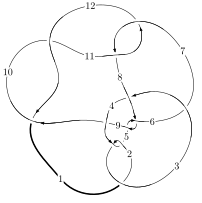
\includegraphics[width=112pt]{../../../GIT/diagram.site/Diagrams/png/2235_12n_0146.png}\\
\ \ \ A knot diagram\footnotemark}&
\allowdisplaybreaks
\textbf{Linearized knot diagam} \\
\cline{2-2}
 &
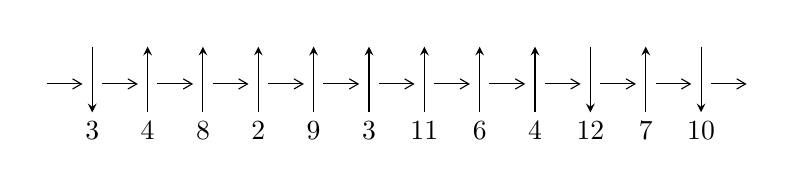
\begin{tikzpicture}[x=20pt, y=17pt]
	% nodes
	\node (C0) at (0, 0) {};
	\node (C1) at (1, 0) {};
	\node (C1U) at (1, +1) {};
	\node (C1D) at (1, -1) {3};

	\node (C2) at (2, 0) {};
	\node (C2U) at (2, +1) {};
	\node (C2D) at (2, -1) {4};

	\node (C3) at (3, 0) {};
	\node (C3U) at (3, +1) {};
	\node (C3D) at (3, -1) {8};

	\node (C4) at (4, 0) {};
	\node (C4U) at (4, +1) {};
	\node (C4D) at (4, -1) {2};

	\node (C5) at (5, 0) {};
	\node (C5U) at (5, +1) {};
	\node (C5D) at (5, -1) {9};

	\node (C6) at (6, 0) {};
	\node (C6U) at (6, +1) {};
	\node (C6D) at (6, -1) {3};

	\node (C7) at (7, 0) {};
	\node (C7U) at (7, +1) {};
	\node (C7D) at (7, -1) {11};

	\node (C8) at (8, 0) {};
	\node (C8U) at (8, +1) {};
	\node (C8D) at (8, -1) {6};

	\node (C9) at (9, 0) {};
	\node (C9U) at (9, +1) {};
	\node (C9D) at (9, -1) {4};

	\node (C10) at (10, 0) {};
	\node (C10U) at (10, +1) {};
	\node (C10D) at (10, -1) {12};

	\node (C11) at (11, 0) {};
	\node (C11U) at (11, +1) {};
	\node (C11D) at (11, -1) {7};

	\node (C12) at (12, 0) {};
	\node (C12U) at (12, +1) {};
	\node (C12D) at (12, -1) {10};
	\node (C13) at (13, 0) {};

	% arrows
	\draw[->,>={angle 60}]
	(C0) edge (C1) (C1) edge (C2) (C2) edge (C3) (C3) edge (C4) (C4) edge (C5) (C5) edge (C6) (C6) edge (C7) (C7) edge (C8) (C8) edge (C9) (C9) edge (C10) (C10) edge (C11) (C11) edge (C12) (C12) edge (C13) ;	\draw[->,>=stealth]
	(C1U) edge (C1D) (C2D) edge (C2U) (C3D) edge (C3U) (C4D) edge (C4U) (C5D) edge (C5U) (C6D) edge (C6U) (C7D) edge (C7U) (C8D) edge (C8U) (C9D) edge (C9U) (C10U) edge (C10D) (C11D) edge (C11U) (C12U) edge (C12D) ;
	\end{tikzpicture} \\
\hhline{~~} \\& 
\textbf{Solving Sequence} \\ \cline{2-2} 
 &
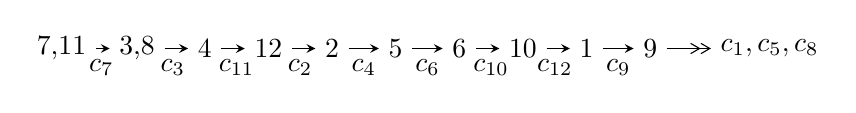
\begin{tikzpicture}[x=23pt, y=7pt]
	% node
	\node (A0) at (-1/8, 0) {7,11};
	\node (A1) at (17/16, 0) {3,8};
	\node (A2) at (17/8, 0) {4};
	\node (A3) at (25/8, 0) {12};
	\node (A4) at (33/8, 0) {2};
	\node (A5) at (41/8, 0) {5};
	\node (A6) at (49/8, 0) {6};
	\node (A7) at (57/8, 0) {10};
	\node (A8) at (65/8, 0) {1};
	\node (A9) at (73/8, 0) {9};
	\node (C1) at (1/2, -1) {$c_{7}$};
	\node (C2) at (13/8, -1) {$c_{3}$};
	\node (C3) at (21/8, -1) {$c_{11}$};
	\node (C4) at (29/8, -1) {$c_{2}$};
	\node (C5) at (37/8, -1) {$c_{4}$};
	\node (C6) at (45/8, -1) {$c_{6}$};
	\node (C7) at (53/8, -1) {$c_{10}$};
	\node (C8) at (61/8, -1) {$c_{12}$};
	\node (C9) at (69/8, -1) {$c_{9}$};
	\node (A10) at (11, 0) {$c_{1},c_{5},c_{8}$};

	% edge
	\draw[->,>=stealth]	
	(A0) edge (A1) (A1) edge (A2) (A2) edge (A3) (A3) edge (A4) (A4) edge (A5) (A5) edge (A6) (A6) edge (A7) (A7) edge (A8) (A8) edge (A9) ;
	\draw[->>,>={angle 60}]	
	(A9) edge (A10);
\end{tikzpicture} \\ 

\end{tabular} \\

\footnotetext{
The image of knot diagram is generated by the software ``\textbf{Draw programme}" developed by Andrew Bartholomew(\url{http://www.layer8.co.uk/maths/draw/index.htm\#Running-draw}), where we modified some parts for our purpose(\url{https://github.com/CATsTAILs/LinksPainter}).
}\phantom \\ \newline 
\centering \textbf{Ideals for irreducible components\footnotemark of $X_{\text{par}}$} 
 
\begin{align*}
I^u_{1}&=\langle 
318706249249855 u^{34}+343308076594525 u^{33}+\cdots+360494352478742 b+533442792596781,\\
\phantom{I^u_{1}}&\phantom{= \langle  }-521798240647102 u^{34}-367409641787037 u^{33}+\cdots+360494352478742 a-422040157543549,\\
\phantom{I^u_{1}}&\phantom{= \langle  }u^{35}+u^{34}+\cdots+4 u+1\rangle \\
I^u_{2}&=\langle 
u^5 a+u^4 a+2 u^5+2 u^3 a+2 u^4+2 u^2 a- u^3+4 a u- u^2+5 b- a+3 u+3,\\
\phantom{I^u_{2}}&\phantom{= \langle  }-2 u^5 a+u^4 a+u^4+u^2 a+u^3+a^2-3 a u+u^2+2 a+1,\;u^6+u^4+2 u^2+1\rangle \\
\\
\end{align*}
\raggedright * 2 irreducible components of $\dim_{\mathbb{C}}=0$, with total 47 representations.\\
\footnotetext{All coefficients of polynomials are rational numbers. But the coefficients are sometimes approximated in decimal forms when there is not enough margin.}
\newpage
\renewcommand{\arraystretch}{1}
\centering \section*{I. $I^u_{1}= \langle 3.19\times10^{14} u^{34}+3.43\times10^{14} u^{33}+\cdots+3.60\times10^{14} b+5.33\times10^{14},\;-5.22\times10^{14} u^{34}-3.67\times10^{14} u^{33}+\cdots+3.60\times10^{14} a-4.22\times10^{14},\;u^{35}+u^{34}+\cdots+4 u+1 \rangle$}
\flushleft \textbf{(i) Arc colorings}\\
\begin{tabular}{m{7pt} m{180pt} m{7pt} m{180pt} }
\flushright $a_{7}=$&$\begin{pmatrix}1\\0\end{pmatrix}$ \\
\flushright $a_{11}=$&$\begin{pmatrix}0\\u\end{pmatrix}$ \\
\flushright $a_{3}=$&$\begin{pmatrix}1.44745 u^{34}+1.01918 u^{33}+\cdots+9.69915 u+1.17073\\-0.884081 u^{34}-0.952326 u^{33}+\cdots-6.17817 u-1.47975\end{pmatrix}$ \\
\flushright $a_{8}=$&$\begin{pmatrix}1\\- u^2\end{pmatrix}$ \\
\flushright $a_{4}=$&$\begin{pmatrix}0.273502 u^{34}+0.0909247 u^{33}+\cdots+3.78660 u+0.119242\\-1.34188 u^{34}-0.869552 u^{33}+\cdots-6.36935 u-1.23406\end{pmatrix}$ \\
\flushright $a_{12}=$&$\begin{pmatrix}u\\u\end{pmatrix}$ \\
\flushright $a_{2}=$&$\begin{pmatrix}3.67262 u^{34}+2.12177 u^{33}+\cdots+15.5688 u+1.41759\\0.828682 u^{34}-0.457894 u^{33}+\cdots+0.578662 u-0.0976132\end{pmatrix}$ \\
\flushright $a_{5}=$&$\begin{pmatrix}-2.45523 u^{34}-2.34388 u^{33}+\cdots-16.0439 u-5.00942\\-1.14001 u^{34}+0.184464 u^{33}+\cdots-1.00983 u+0.111350\end{pmatrix}$ \\
\flushright $a_{6}=$&$\begin{pmatrix}-1.71137 u^{34}-0.579700 u^{33}+\cdots-0.908428 u+1.59802\\-1.58640 u^{34}-0.248141 u^{33}+\cdots-3.92323 u-0.309741\end{pmatrix}$ \\
\flushright $a_{10}=$&$\begin{pmatrix}u^3\\u^3+u\end{pmatrix}$ \\
\flushright $a_{1}=$&$\begin{pmatrix}u^5+u\\u^5+u^3+u\end{pmatrix}$ \\
\flushright $a_{9}=$&$\begin{pmatrix}1.44922 u^{34}-0.334990 u^{33}+\cdots+3.36424 u+0.0154970\\-1.05881 u^{34}-1.67916 u^{33}+\cdots-7.41997 u-2.22848\end{pmatrix}$\\&\end{tabular}
\flushleft \textbf{(ii) Obstruction class $= -1$}\\~\\
\flushleft \textbf{(iii) Cusp Shapes $= \frac{684142960707262}{180247176239371} u^{34}+\frac{484025290669977}{180247176239371} u^{33}+\cdots+\frac{5236709331027379}{180247176239371} u+\frac{2961609232527520}{180247176239371}$}\\~\\
\newpage\renewcommand{\arraystretch}{1}
\flushleft \textbf{(iv) u-Polynomials at the component}\newline \\
\begin{tabular}{m{50pt}|m{274pt}}
Crossings & \hspace{64pt}u-Polynomials at each crossing \\
\hline $$\begin{aligned}c_{1}\end{aligned}$$&$\begin{aligned}
&u^{35}+49 u^{34}+\cdots-74 u-1
\end{aligned}$\\
\hline $$\begin{aligned}c_{2},c_{4}\end{aligned}$$&$\begin{aligned}
&u^{35}-7 u^{34}+\cdots+10 u-1
\end{aligned}$\\
\hline $$\begin{aligned}c_{3}\end{aligned}$$&$\begin{aligned}
&u^{35}+u^{34}+\cdots-4 u-1
\end{aligned}$\\
\hline $$\begin{aligned}c_{5},c_{8}\end{aligned}$$&$\begin{aligned}
&u^{35}+u^{34}+\cdots-20 u-25
\end{aligned}$\\
\hline $$\begin{aligned}c_{6}\end{aligned}$$&$\begin{aligned}
&u^{35}+u^{34}+\cdots-6812 u-1859
\end{aligned}$\\
\hline $$\begin{aligned}c_{7},c_{11}\end{aligned}$$&$\begin{aligned}
&u^{35}- u^{34}+\cdots+4 u-1
\end{aligned}$\\
\hline $$\begin{aligned}c_{9}\end{aligned}$$&$\begin{aligned}
&u^{35}+u^{34}+\cdots+18028 u-13207
\end{aligned}$\\
\hline $$\begin{aligned}c_{10},c_{12}\end{aligned}$$&$\begin{aligned}
&u^{35}+15 u^{34}+\cdots-4 u-1
\end{aligned}$\\
\hline
\end{tabular}\\~\\
\newpage\renewcommand{\arraystretch}{1}
\flushleft \textbf{(v) Riley Polynomials at the component}\newline \\
\begin{tabular}{m{50pt}|m{274pt}}
Crossings & \hspace{64pt}Riley Polynomials at each crossing \\
\hline $$\begin{aligned}c_{1}\end{aligned}$$&$\begin{aligned}
&y^{35}-119 y^{34}+\cdots-5290 y-1
\end{aligned}$\\
\hline $$\begin{aligned}c_{2},c_{4}\end{aligned}$$&$\begin{aligned}
&y^{35}+49 y^{34}+\cdots-74 y-1
\end{aligned}$\\
\hline $$\begin{aligned}c_{3}\end{aligned}$$&$\begin{aligned}
&y^{35}-7 y^{34}+\cdots+10 y-1
\end{aligned}$\\
\hline $$\begin{aligned}c_{5},c_{8}\end{aligned}$$&$\begin{aligned}
&y^{35}+51 y^{34}+\cdots+1100 y-625
\end{aligned}$\\
\hline $$\begin{aligned}c_{6}\end{aligned}$$&$\begin{aligned}
&y^{35}+31 y^{34}+\cdots-14003002 y-3455881
\end{aligned}$\\
\hline $$\begin{aligned}c_{7},c_{11}\end{aligned}$$&$\begin{aligned}
&y^{35}+15 y^{34}+\cdots-4 y-1
\end{aligned}$\\
\hline $$\begin{aligned}c_{9}\end{aligned}$$&$\begin{aligned}
&y^{35}+87 y^{34}+\cdots+3505280798 y-174424849
\end{aligned}$\\
\hline $$\begin{aligned}c_{10},c_{12}\end{aligned}$$&$\begin{aligned}
&y^{35}+15 y^{34}+\cdots+52 y-1
\end{aligned}$\\
\hline
\end{tabular}\\~\\
\newpage\flushleft \textbf{(vi) Complex Volumes and Cusp Shapes}
$$\begin{array}{c|c|c}  
\text{Solutions to }I^u_{1}& \I (\text{vol} + \sqrt{-1}CS) & \text{Cusp shape}\\
 \hline 
\begin{aligned}
u &= -0.198898 + 0.912281 I \\
a &= -0.21214 + 1.53304 I \\
b &= -0.221795 + 0.558249 I\end{aligned}
 & -1.69730 - 1.70582 I & \phantom{-}2.23067 + 4.51797 I \\ \hline\begin{aligned}
u &= -0.198898 - 0.912281 I \\
a &= -0.21214 - 1.53304 I \\
b &= -0.221795 - 0.558249 I\end{aligned}
 & -1.69730 + 1.70582 I & \phantom{-}2.23067 - 4.51797 I \\ \hline\begin{aligned}
u &= \phantom{-}0.706440 + 0.807195 I \\
a &= -0.819135 + 0.009162 I \\
b &= -1.02181 + 1.22008 I\end{aligned}
 & \phantom{-}3.47975 + 0.18002 I & \phantom{-}12.74797 + 1.67339 I \\ \hline\begin{aligned}
u &= \phantom{-}0.706440 - 0.807195 I \\
a &= -0.819135 - 0.009162 I \\
b &= -1.02181 - 1.22008 I\end{aligned}
 & \phantom{-}3.47975 - 0.18002 I & \phantom{-}12.74797 - 1.67339 I \\ \hline\begin{aligned}
u &= \phantom{-}0.987560 + 0.453130 I \\
a &= -0.479255 + 0.468522 I \\
b &= -0.105454 - 0.947398 I\end{aligned}
 & -11.79900 + 0.75958 I & \phantom{-}4.27228 - 1.73468 I \\ \hline\begin{aligned}
u &= \phantom{-}0.987560 - 0.453130 I \\
a &= -0.479255 - 0.468522 I \\
b &= -0.105454 + 0.947398 I\end{aligned}
 & -11.79900 - 0.75958 I & \phantom{-}4.27228 + 1.73468 I \\ \hline\begin{aligned}
u &= -0.419414 + 1.027600 I \\
a &= \phantom{-}0.988734 + 0.871634 I \\
b &= -0.885142 + 0.876577 I\end{aligned}
 & -3.34462 - 0.85949 I & \phantom{-}2.28344 + 2.34599 I \\ \hline\begin{aligned}
u &= -0.419414 - 1.027600 I \\
a &= \phantom{-}0.988734 - 0.871634 I \\
b &= -0.885142 - 0.876577 I\end{aligned}
 & -3.34462 + 0.85949 I & \phantom{-}2.28344 - 2.34599 I \\ \hline\begin{aligned}
u &= -0.980550 + 0.531852 I \\
a &= -0.521288 + 0.398754 I \\
b &= -1.11162 - 1.73230 I\end{aligned}
 & -11.27240 + 6.32601 I & \phantom{-}4.80195 - 2.51177 I \\ \hline\begin{aligned}
u &= -0.980550 - 0.531852 I \\
a &= -0.521288 - 0.398754 I \\
b &= -1.11162 + 1.73230 I\end{aligned}
 & -11.27240 - 6.32601 I & \phantom{-}4.80195 + 2.51177 I\\
 \hline 
 \end{array}$$\newpage$$\begin{array}{c|c|c}  
\text{Solutions to }I^u_{1}& \I (\text{vol} + \sqrt{-1}CS) & \text{Cusp shape}\\
 \hline 
\begin{aligned}
u &= -0.736027 + 0.839562 I \\
a &= \phantom{-}0.102548 - 0.713671 I \\
b &= \phantom{-}1.199180 + 0.185153 I\end{aligned}
 & \phantom{-}1.37968 - 2.70140 I & \phantom{-}5.99641 + 3.98735 I \\ \hline\begin{aligned}
u &= -0.736027 - 0.839562 I \\
a &= \phantom{-}0.102548 + 0.713671 I \\
b &= \phantom{-}1.199180 - 0.185153 I\end{aligned}
 & \phantom{-}1.37968 + 2.70140 I & \phantom{-}5.99641 - 3.98735 I \\ \hline\begin{aligned}
u &= \phantom{-}0.315075 + 1.089710 I \\
a &= \phantom{-}1.26686 - 0.81863 I \\
b &= \phantom{-}0.367656 - 0.856256 I\end{aligned}
 & -5.45958 + 0.17425 I & -0.394097 - 0.771153 I \\ \hline\begin{aligned}
u &= \phantom{-}0.315075 - 1.089710 I \\
a &= \phantom{-}1.26686 + 0.81863 I \\
b &= \phantom{-}0.367656 + 0.856256 I\end{aligned}
 & -5.45958 - 0.17425 I & -0.394097 + 0.771153 I \\ \hline\begin{aligned}
u &= -0.497697 + 1.028650 I \\
a &= -0.97579 - 1.97047 I \\
b &= \phantom{-}0.04867 - 2.11164 I\end{aligned}
 & -2.82734 - 5.45471 I & \phantom{-}3.55595 + 5.75230 I \\ \hline\begin{aligned}
u &= -0.497697 - 1.028650 I \\
a &= -0.97579 + 1.97047 I \\
b &= \phantom{-}0.04867 + 2.11164 I\end{aligned}
 & -2.82734 + 5.45471 I & \phantom{-}3.55595 - 5.75230 I \\ \hline\begin{aligned}
u &= \phantom{-}0.709383 + 0.907946 I \\
a &= \phantom{-}1.10452 - 1.42282 I \\
b &= -0.57945 - 1.52300 I\end{aligned}
 & \phantom{-}3.18411 + 5.24743 I & \phantom{-}11.9368 - 7.8147 I \\ \hline\begin{aligned}
u &= \phantom{-}0.709383 - 0.907946 I \\
a &= \phantom{-}1.10452 + 1.42282 I \\
b &= -0.57945 + 1.52300 I\end{aligned}
 & \phantom{-}3.18411 - 5.24743 I & \phantom{-}11.9368 + 7.8147 I \\ \hline\begin{aligned}
u &= -0.699352 + 0.916434 I \\
a &= -0.482223 - 0.911197 I \\
b &= \phantom{-}0.814763 - 0.513730 I\end{aligned}
 & \phantom{-}1.15135 - 2.78726 I & \phantom{-}4.50130 + 1.74578 I \\ \hline\begin{aligned}
u &= -0.699352 - 0.916434 I \\
a &= -0.482223 + 0.911197 I \\
b &= \phantom{-}0.814763 + 0.513730 I\end{aligned}
 & \phantom{-}1.15135 + 2.78726 I & \phantom{-}4.50130 - 1.74578 I\\
 \hline 
 \end{array}$$\newpage$$\begin{array}{c|c|c}  
\text{Solutions to }I^u_{1}& \I (\text{vol} + \sqrt{-1}CS) & \text{Cusp shape}\\
 \hline 
\begin{aligned}
u &= \phantom{-}0.530985 + 1.088540 I \\
a &= -0.22183 + 1.99595 I \\
b &= \phantom{-}1.28242 + 1.15849 I\end{aligned}
 & -4.02551 + 7.04503 I & \phantom{-}2.61668 - 6.73357 I \\ \hline\begin{aligned}
u &= \phantom{-}0.530985 - 1.088540 I \\
a &= -0.22183 - 1.99595 I \\
b &= \phantom{-}1.28242 - 1.15849 I\end{aligned}
 & -4.02551 - 7.04503 I & \phantom{-}2.61668 + 6.73357 I \\ \hline\begin{aligned}
u &= -0.423966 + 0.601689 I \\
a &= \phantom{-}1.84029 + 1.10036 I \\
b &= \phantom{-}0.76833 + 1.48875 I\end{aligned}
 & -1.39115 + 1.47351 I & \phantom{-}7.00418 - 0.38394 I \\ \hline\begin{aligned}
u &= -0.423966 - 0.601689 I \\
a &= \phantom{-}1.84029 - 1.10036 I \\
b &= \phantom{-}0.76833 - 1.48875 I\end{aligned}
 & -1.39115 - 1.47351 I & \phantom{-}7.00418 + 0.38394 I \\ \hline\begin{aligned}
u &= \phantom{-}0.039193 + 1.312350 I \\
a &= -0.63914 - 1.68853 I \\
b &= -0.25205 - 1.80126 I\end{aligned}
 & -18.4544 + 3.7875 I & \phantom{-}0.15008 - 2.18954 I \\ \hline\begin{aligned}
u &= \phantom{-}0.039193 - 1.312350 I \\
a &= -0.63914 + 1.68853 I \\
b &= -0.25205 + 1.80126 I\end{aligned}
 & -18.4544 - 3.7875 I & \phantom{-}0.15008 + 2.18954 I \\ \hline\begin{aligned}
u &= \phantom{-}0.571745 + 0.303555 I \\
a &= -0.423437 + 0.372340 I \\
b &= \phantom{-}0.988498 - 0.658097 I\end{aligned}
 & -1.87714 - 2.57774 I & \phantom{-}5.81524 + 3.28141 I \\ \hline\begin{aligned}
u &= \phantom{-}0.571745 - 0.303555 I \\
a &= -0.423437 - 0.372340 I \\
b &= \phantom{-}0.988498 + 0.658097 I\end{aligned}
 & -1.87714 + 2.57774 I & \phantom{-}5.81524 - 3.28141 I \\ \hline\begin{aligned}
u &= -0.719484 + 1.148000 I \\
a &= \phantom{-}0.88560 + 1.88560 I \\
b &= -1.30329 + 2.06739 I\end{aligned}
 & -13.1891 - 12.5329 I & \phantom{-}3.21529 + 6.50684 I \\ \hline\begin{aligned}
u &= -0.719484 - 1.148000 I \\
a &= \phantom{-}0.88560 - 1.88560 I \\
b &= -1.30329 - 2.06739 I\end{aligned}
 & -13.1891 + 12.5329 I & \phantom{-}3.21529 - 6.50684 I\\
 \hline 
 \end{array}$$\newpage$$\begin{array}{c|c|c}  
\text{Solutions to }I^u_{1}& \I (\text{vol} + \sqrt{-1}CS) & \text{Cusp shape}\\
 \hline 
\begin{aligned}
u &= \phantom{-}0.679877 + 1.180490 I \\
a &= -1.009050 + 0.279744 I \\
b &= \phantom{-}0.353942 + 0.804369 I\end{aligned}
 & -14.0684 + 5.3198 I & \phantom{-}2.14370 - 2.29588 I \\ \hline\begin{aligned}
u &= \phantom{-}0.679877 - 1.180490 I \\
a &= -1.009050 - 0.279744 I \\
b &= \phantom{-}0.353942 - 0.804369 I\end{aligned}
 & -14.0684 - 5.3198 I & \phantom{-}2.14370 + 2.29588 I \\ \hline\begin{aligned}
u &= -0.191898 + 0.428395 I \\
a &= -0.57700 + 2.20593 I \\
b &= \phantom{-}0.393176 - 0.360559 I\end{aligned}
 & -1.57284 - 2.29524 I & \phantom{-}6.98932 + 5.13879 I \\ \hline\begin{aligned}
u &= -0.191898 - 0.428395 I \\
a &= -0.57700 - 2.20593 I \\
b &= \phantom{-}0.393176 + 0.360559 I\end{aligned}
 & -1.57284 + 2.29524 I & \phantom{-}6.98932 - 5.13879 I \\ \hline\begin{aligned}
u &= -0.345944\phantom{ +0.000000I} \\
a &= -0.656543\phantom{ +0.000000I} \\
b &= -0.472048\phantom{ +0.000000I}\end{aligned}
 & \phantom{-}0.719348\phantom{ +0.000000I} & \phantom{-}14.2660\phantom{ +0.000000I}\\
 \hline 
 \end{array}$$\newpage\newpage\renewcommand{\arraystretch}{1}
\centering \section*{II. $I^u_{2}= \langle u^5 a+2 u^5+\cdots- a+3,\;-2 u^5 a+u^4 a+\cdots+2 a+1,\;u^6+u^4+2 u^2+1 \rangle$}
\flushleft \textbf{(i) Arc colorings}\\
\begin{tabular}{m{7pt} m{180pt} m{7pt} m{180pt} }
\flushright $a_{7}=$&$\begin{pmatrix}1\\0\end{pmatrix}$ \\
\flushright $a_{11}=$&$\begin{pmatrix}0\\u\end{pmatrix}$ \\
\flushright $a_{3}=$&$\begin{pmatrix}a\\-\frac{1}{5} u^5 a-\frac{2}{5} u^5+\cdots+\frac{1}{5} a-\frac{3}{5}\end{pmatrix}$ \\
\flushright $a_{8}=$&$\begin{pmatrix}1\\- u^2\end{pmatrix}$ \\
\flushright $a_{4}=$&$\begin{pmatrix}-\frac{1}{5} u^5 a-\frac{2}{5} u^5+\cdots+\frac{6}{5} a-\frac{3}{5}\\- u^4 a- u^5- u^4- u^2 a- a u- u-1\end{pmatrix}$ \\
\flushright $a_{12}=$&$\begin{pmatrix}u\\u\end{pmatrix}$ \\
\flushright $a_{2}=$&$\begin{pmatrix}\frac{4}{5} u^5 a+\frac{8}{5} u^5+\cdots+\frac{1}{5} a-\frac{3}{5}\\2 u^5+2 u^3+2 u-1\end{pmatrix}$ \\
\flushright $a_{5}=$&$\begin{pmatrix}- u^5- u\\- u^5- u^3- u\end{pmatrix}$ \\
\flushright $a_{6}=$&$\begin{pmatrix}\frac{7}{5} u^5 a+\frac{4}{5} u^5+\cdots-\frac{2}{5} a+\frac{1}{5}\\\frac{3}{5} u^5 a+\frac{11}{5} u^5+\cdots+\frac{2}{5} a-\frac{1}{5}\end{pmatrix}$ \\
\flushright $a_{10}=$&$\begin{pmatrix}u^3\\u^3+u\end{pmatrix}$ \\
\flushright $a_{1}=$&$\begin{pmatrix}u^5+u\\u^5+u^3+u\end{pmatrix}$ \\
\flushright $a_{9}=$&$\begin{pmatrix}\frac{1}{5} u^5 a-\frac{8}{5} u^5+\cdots+\frac{4}{5} a+\frac{8}{5}\\\frac{4}{5} u^5 a-\frac{2}{5} u^5+\cdots+\frac{1}{5} a+\frac{2}{5}\end{pmatrix}$\\&\end{tabular}
\flushleft \textbf{(ii) Obstruction class $= 1$}\\~\\
\flushleft \textbf{(iii) Cusp Shapes $= -\frac{8}{5} u^5 a+\frac{12}{5} u^4 a-\frac{16}{5} u^5-\frac{16}{5} u^3 a-\frac{16}{5} u^4+\frac{4}{5} u^2 a-\frac{12}{5} u^3-\frac{12}{5} a u-\frac{12}{5} u^2+\frac{8}{5} a-\frac{24}{5} u-\frac{4}{5}$}\\~\\
\newpage\renewcommand{\arraystretch}{1}
\flushleft \textbf{(iv) u-Polynomials at the component}\newline \\
\begin{tabular}{m{50pt}|m{274pt}}
Crossings & \hspace{64pt}u-Polynomials at each crossing \\
\hline $$\begin{aligned}c_{1},c_{4}\end{aligned}$$&$\begin{aligned}
&(u^2- u+1)^6
\end{aligned}$\\
\hline $$\begin{aligned}c_{2}\end{aligned}$$&$\begin{aligned}
&(u^2+u+1)^6
\end{aligned}$\\
\hline $$\begin{aligned}c_{3}\end{aligned}$$&$\begin{aligned}
&(u^4- u^2+1)^3
\end{aligned}$\\
\hline $$\begin{aligned}c_{5},c_{8}\end{aligned}$$&$\begin{aligned}
&(u^2+1)^6
\end{aligned}$\\
\hline $$\begin{aligned}c_{6}\end{aligned}$$&$\begin{aligned}
&u^{12}+6 u^{11}+\cdots-2 u+1
\end{aligned}$\\
\hline $$\begin{aligned}c_{7},c_{11}\end{aligned}$$&$\begin{aligned}
&(u^6+u^4+2 u^2+1)^2
\end{aligned}$\\
\hline $$\begin{aligned}c_{9}\end{aligned}$$&$\begin{aligned}
&u^{12}-2 u^{11}+\cdots-4 u+1
\end{aligned}$\\
\hline $$\begin{aligned}c_{10}\end{aligned}$$&$\begin{aligned}
&(u^3- u^2+2 u-1)^4
\end{aligned}$\\
\hline $$\begin{aligned}c_{12}\end{aligned}$$&$\begin{aligned}
&(u^3+u^2+2 u+1)^4
\end{aligned}$\\
\hline
\end{tabular}\\~\\
\newpage\renewcommand{\arraystretch}{1}
\flushleft \textbf{(v) Riley Polynomials at the component}\newline \\
\begin{tabular}{m{50pt}|m{274pt}}
Crossings & \hspace{64pt}Riley Polynomials at each crossing \\
\hline $$\begin{aligned}c_{1},c_{2},c_{4}\end{aligned}$$&$\begin{aligned}
&(y^2+y+1)^6
\end{aligned}$\\
\hline $$\begin{aligned}c_{3}\end{aligned}$$&$\begin{aligned}
&(y^2- y+1)^6
\end{aligned}$\\
\hline $$\begin{aligned}c_{5},c_{8}\end{aligned}$$&$\begin{aligned}
&(y+1)^{12}
\end{aligned}$\\
\hline $$\begin{aligned}c_{6}\end{aligned}$$&$\begin{aligned}
&y^{12}+12 y^{11}+\cdots+6 y+1
\end{aligned}$\\
\hline $$\begin{aligned}c_{7},c_{11}\end{aligned}$$&$\begin{aligned}
&(y^3+y^2+2 y+1)^4
\end{aligned}$\\
\hline $$\begin{aligned}c_{9}\end{aligned}$$&$\begin{aligned}
&y^{12}-12 y^{11}+\cdots-6 y+1
\end{aligned}$\\
\hline $$\begin{aligned}c_{10},c_{12}\end{aligned}$$&$\begin{aligned}
&(y^3+3 y^2+2 y-1)^4
\end{aligned}$\\
\hline
\end{tabular}\\~\\
\newpage\flushleft \textbf{(vi) Complex Volumes and Cusp Shapes}
$$\begin{array}{c|c|c}  
\text{Solutions to }I^u_{2}& \I (\text{vol} + \sqrt{-1}CS) & \text{Cusp shape}\\
 \hline 
\begin{aligned}
u &= \phantom{-}0.744862 + 0.877439 I \\
a &= -1.093800 - 0.182501 I \\
b &= -1.33984 + 1.89050 I\end{aligned}
 & \phantom{-}1.37919 - 4.85801 I & \phantom{-}5.50976 + 0.48465 I \\ \hline\begin{aligned}
u &= \phantom{-}0.744862 + 0.877439 I \\
a &= \phantom{-}1.71610 - 1.68492 I \\
b &= -0.96731 - 2.10558 I\end{aligned}
 & \phantom{-}1.37919 - 0.79824 I & \phantom{-}5.50976 - 6.44355 I \\ \hline\begin{aligned}
u &= \phantom{-}0.744862 - 0.877439 I \\
a &= -1.093800 + 0.182501 I \\
b &= -1.33984 - 1.89050 I\end{aligned}
 & \phantom{-}1.37919 + 4.85801 I & \phantom{-}5.50976 - 0.48465 I \\ \hline\begin{aligned}
u &= \phantom{-}0.744862 - 0.877439 I \\
a &= \phantom{-}1.71610 + 1.68492 I \\
b &= -0.96731 + 2.10558 I\end{aligned}
 & \phantom{-}1.37919 + 0.79824 I & \phantom{-}5.50976 + 6.44355 I \\ \hline\begin{aligned}
u &= -0.744862 + 0.877439 I \\
a &= -0.548527 - 0.727778 I \\
b &= -0.032694 - 0.373532 I\end{aligned}
 & \phantom{-}1.37919 + 0.79824 I & \phantom{-}5.50976 + 6.44355 I \\ \hline\begin{aligned}
u &= -0.744862 + 0.877439 I \\
a &= -0.318896 + 0.350078 I \\
b &= \phantom{-}0.339835 + 0.158452 I\end{aligned}
 & \phantom{-}1.37919 + 4.85801 I & \phantom{-}5.50976 - 0.48465 I \\ \hline\begin{aligned}
u &= -0.744862 - 0.877439 I \\
a &= -0.548527 + 0.727778 I \\
b &= -0.032694 + 0.373532 I\end{aligned}
 & \phantom{-}1.37919 - 0.79824 I & \phantom{-}5.50976 - 6.44355 I \\ \hline\begin{aligned}
u &= -0.744862 - 0.877439 I \\
a &= -0.318896 - 0.350078 I \\
b &= \phantom{-}0.339835 - 0.158452 I\end{aligned}
 & \phantom{-}1.37919 - 4.85801 I & \phantom{-}5.50976 + 0.48465 I \\ \hline\begin{aligned}
u &= \phantom{-0.000000 -}0.754878 I \\
a &= -0.223696 - 0.142330 I \\
b &= -0.993496 - 0.581105 I\end{aligned}
 & -2.75839 + 2.02988 I & -1.01951 - 3.46410 I \\ \hline\begin{aligned}
u &= \phantom{-0.000000 -}0.754878 I \\
a &= -1.53118 + 2.89721 I \\
b &= -0.006504 + 1.150950 I\end{aligned}
 & -2.75839 - 2.02988 I & -1.01951 + 3.46410 I\\
 \hline 
 \end{array}$$\newpage$$\begin{array}{c|c|c}  
\text{Solutions to }I^u_{2}& \I (\text{vol} + \sqrt{-1}CS) & \text{Cusp shape}\\
 \hline 
\begin{aligned}
u &= \phantom{-0.000000 } -0.754878 I \\
a &= -0.223696 + 0.142330 I \\
b &= -0.993496 + 0.581105 I\end{aligned}
 & -2.75839 - 2.02988 I & -1.01951 + 3.46410 I \\ \hline\begin{aligned}
u &= \phantom{-0.000000 } -0.754878 I \\
a &= -1.53118 - 2.89721 I \\
b &= -0.006504 - 1.150950 I\end{aligned}
 & -2.75839 + 2.02988 I & -1.01951 - 3.46410 I\\
 \hline 
 \end{array}$$\newpage
\newpage\renewcommand{\arraystretch}{1}
\centering \section*{ III. u-Polynomials}
\begin{tabular}{m{50pt}|m{274pt}}
Crossings & \hspace{64pt}u-Polynomials at each crossing \\
\hline $$\begin{aligned}c_{1}\end{aligned}$$&$\begin{aligned}
&((u^2- u+1)^6)(u^{35}+49 u^{34}+\cdots-74 u-1)
\end{aligned}$\\
\hline $$\begin{aligned}c_{2}\end{aligned}$$&$\begin{aligned}
&((u^2+u+1)^6)(u^{35}-7 u^{34}+\cdots+10 u-1)
\end{aligned}$\\
\hline $$\begin{aligned}c_{3}\end{aligned}$$&$\begin{aligned}
&((u^4- u^2+1)^3)(u^{35}+u^{34}+\cdots-4 u-1)
\end{aligned}$\\
\hline $$\begin{aligned}c_{4}\end{aligned}$$&$\begin{aligned}
&((u^2- u+1)^6)(u^{35}-7 u^{34}+\cdots+10 u-1)
\end{aligned}$\\
\hline $$\begin{aligned}c_{5},c_{8}\end{aligned}$$&$\begin{aligned}
&((u^2+1)^6)(u^{35}+u^{34}+\cdots-20 u-25)
\end{aligned}$\\
\hline $$\begin{aligned}c_{6}\end{aligned}$$&$\begin{aligned}
&(u^{12}+6 u^{11}+\cdots-2 u+1)(u^{35}+u^{34}+\cdots-6812 u-1859)
\end{aligned}$\\
\hline $$\begin{aligned}c_{7},c_{11}\end{aligned}$$&$\begin{aligned}
&((u^6+u^4+2 u^2+1)^2)(u^{35}- u^{34}+\cdots+4 u-1)
\end{aligned}$\\
\hline $$\begin{aligned}c_{9}\end{aligned}$$&$\begin{aligned}
&(u^{12}-2 u^{11}+\cdots-4 u+1)(u^{35}+u^{34}+\cdots+18028 u-13207)
\end{aligned}$\\
\hline $$\begin{aligned}c_{10}\end{aligned}$$&$\begin{aligned}
&((u^3- u^2+2 u-1)^4)(u^{35}+15 u^{34}+\cdots-4 u-1)
\end{aligned}$\\
\hline $$\begin{aligned}c_{12}\end{aligned}$$&$\begin{aligned}
&((u^3+u^2+2 u+1)^4)(u^{35}+15 u^{34}+\cdots-4 u-1)
\end{aligned}$\\
\hline
\end{tabular}\newpage\renewcommand{\arraystretch}{1}
\centering \section*{ IV. Riley Polynomials}
\begin{tabular}{m{50pt}|m{274pt}}
Crossings & \hspace{64pt}Riley Polynomials at each crossing \\
\hline $$\begin{aligned}c_{1}\end{aligned}$$&$\begin{aligned}
&((y^2+y+1)^6)(y^{35}-119 y^{34}+\cdots-5290 y-1)
\end{aligned}$\\
\hline $$\begin{aligned}c_{2},c_{4}\end{aligned}$$&$\begin{aligned}
&((y^2+y+1)^6)(y^{35}+49 y^{34}+\cdots-74 y-1)
\end{aligned}$\\
\hline $$\begin{aligned}c_{3}\end{aligned}$$&$\begin{aligned}
&((y^2- y+1)^6)(y^{35}-7 y^{34}+\cdots+10 y-1)
\end{aligned}$\\
\hline $$\begin{aligned}c_{5},c_{8}\end{aligned}$$&$\begin{aligned}
&((y+1)^{12})(y^{35}+51 y^{34}+\cdots+1100 y-625)
\end{aligned}$\\
\hline $$\begin{aligned}c_{6}\end{aligned}$$&$\begin{aligned}
&(y^{12}+12 y^{11}+\cdots+6 y+1)\\
&\cdot(y^{35}+31 y^{34}+\cdots-14003002 y-3455881)
\end{aligned}$\\
\hline $$\begin{aligned}c_{7},c_{11}\end{aligned}$$&$\begin{aligned}
&((y^3+y^2+2 y+1)^4)(y^{35}+15 y^{34}+\cdots-4 y-1)
\end{aligned}$\\
\hline $$\begin{aligned}c_{9}\end{aligned}$$&$\begin{aligned}
&(y^{12}-12 y^{11}+\cdots-6 y+1)\\
&\cdot(y^{35}+87 y^{34}+\cdots+3505280798 y-174424849)
\end{aligned}$\\
\hline $$\begin{aligned}c_{10},c_{12}\end{aligned}$$&$\begin{aligned}
&((y^3+3 y^2+2 y-1)^4)(y^{35}+15 y^{34}+\cdots+52 y-1)
\end{aligned}$\\
\hline
\end{tabular}
\vskip 2pc
\end{document}